\documentclass[manuscript,screen]{acmart}

\setcopyright{none}
\settopmatter{printacmref=false}
\renewcommand\footnotetextcopyrightpermission[1]{}
\pagestyle{plain}

\usepackage{booktabs}
\usepackage{longtable}
\usepackage{tabularx}
\usepackage{enumitem}
\usepackage{hyperref}
\usepackage{array}

\title{A Reproduction Study of GuP for Exact Subgraph Matching}

\author{Yi Zha}
\affiliation{%
  \institution{Tsinghua University}
  \city{Beijing}
  \country{China}}
\email{chay22@mails.tsinghua.edu.cn}

\author{Jinpeng Wang}
\affiliation{%
  \institution{Tsinghua University}
  \city{Beijing}
  \country{China}}
\email{wjp21@mails.tsinghua.edu.cn}

\begin{document}

\begin{abstract}
This paper presents a reproduction study of GuP, an exact subgraph matching method based on guard-based pruning. We implemented a correctness-oriented baseline matcher and extended it with a \emph{GUP-lite} design that supports reservation-based pruning, nogood-based pruning, metric collection, and filtering-strategy ablation. The study includes a literature taxonomy, a clear statement of reproduction scope, experiments on three successful datasets (Yeast, Human, and HPRD), three optional extensions---query-result reuse, incremental result maintenance under single-edge data-graph updates, and subgraph homomorphism---and a time-boxed boundary evaluation on WordNet and Patents. Reservation-based pruning is the main source of reduction on the six fixed dense-4 workloads, while post-fix dense-8 validation shows that nogood reuse can become dominant when many histories induce the same failing future subproblem. The Python implementation still shows a clear scalability boundary.
\end{abstract}

\maketitle

\keywords{exact subgraph matching, guard-based pruning, reproduction study, graph query processing}
\ccsdesc[500]{Information systems~Graph-based database models}
\ccsdesc[300]{Theory of computation~Graph algorithms analysis}


\section{Introduction}

Exact subgraph matching is a fundamental graph query problem with applications in social-network analysis, biological interaction analysis, fraud detection, and graph database systems. Given a large vertex-labeled data graph and a smaller query graph, the goal is to enumerate all injective mappings that preserve both labels and edges. Because the search space grows rapidly with query size, practical systems rely heavily on candidate filtering, matching-order optimization, and state-aware pruning.

In this project, we reproduce \emph{GuP}, a recent exact subgraph matching method based on guard-based pruning~\cite{arai2023gup}. GuP introduces two complementary pruning ideas: reservation guards, which propagate injectivity-related constraints to earlier search steps, and nogood guards, which attempt to reuse dead-end information discovered during the search. These mechanisms are designed to reduce futile recursive exploration while preserving exactness.

The goal of this course project is not only to obtain a runnable implementation, but also to present a clear and complete analysis. Accordingly, besides implementing and evaluating a correctness-oriented reproduction of GuP, we organize the report around four core components: literature review and taxonomy, reproduction of one selected paper, required experiments on multiple datasets with specified metrics, and ablation of filtering strategies.

\subsection{Project Scope}

Our implementation follows a staged strategy. We first build a baseline depth-first backtracking matcher, then add GuP-inspired reservation and nogood guards, and finally evaluate the resulting variants under a shared metric framework. The resulting system is still a course-project reproduction rather than a line-by-line reimplementation of the authors' production code, but it already captures the main algorithmic components needed for comparative analysis.

\subsection{Report Organization and Grading-Item Mapping}

Table~\ref{tab:rubric-mapping} summarizes how the report structure aligns with the required grading items.

\begin{table}[t]
  \caption{Mapping from the grading rubric to the report structure.}
  \label{tab:rubric-mapping}
  \centering
  \footnotesize
  \setlength{\tabcolsep}{4pt}
  \begin{tabularx}{\columnwidth}{>{\raggedright\arraybackslash}p{0.18\columnwidth} >{\raggedright\arraybackslash}p{0.26\columnwidth} >{\raggedright\arraybackslash}X}
    \toprule
    Grading item & Report sections & Main evidence \\
    \midrule
    Literature review (15 pts) & Secs.~\ref{sec:lit-review}; Tab.~\ref{tab:taxonomy} & Taxonomy and positioning of GuP \\
    Paper reproduction (20 pts) & Secs.~\ref{sec:paper-idea}, \ref{sec:impl-details}; Tab.~\ref{tab:repro-scope} & Reproduced components and scope boundary \\
    Required experiments (20 pts) & Secs.~\ref{sec:exp-setup}, \ref{sec:exp-results}; Tabs.~\ref{tab:dataset-summary}, \ref{tab:required-metrics}, \ref{tab:boundary-datasets} & Runtime, result mappings, partial mappings, and paper-filtered partial mappings \\
    Strategy ablation (15 pts) & Sec.~\ref{sec:ablation}; Tabs.~\ref{tab:strategy-switch}, \ref{tab:ablation-results} & Guard on/off comparison and contribution analysis \\
    \bottomrule
  \end{tabularx}
\end{table}

The remainder of the report is organized as follows. Section~\ref{sec:lit-review} reviews the literature and builds a taxonomy for exact subgraph matching. Sections~\ref{sec:problem-def}--\ref{sec:impl-details} define the problem, summarize GuP, and describe the reproduced system. Sections~\ref{sec:exp-setup}--\ref{sec:ablation} present the required experiments and the ablation study. Section~\ref{sec:conclusion} concludes with a brief development-history discussion and personal reflection.

\section{Literature Review and Multi-dimensional Taxonomy}
\label{sec:lit-review}

Exact subgraph matching has been studied for more than one research generation, and representative progress has appeared from both the database and graph-algorithm communities. Prior work does not advance along a single axis: some methods emphasize aggressive candidate-space reduction before backtracking begins, some optimize the search order to expose contradictions earlier, some reuse dead-end information to avoid repeating equivalent failures, and others redesign the whole execution pipeline around candidate representation and set operations~\cite{he2008graphql,han2019daf,sun2020study,sun2021rapidmatch,kim2022veq,arai2023gup}. Therefore, a meaningful literature review for this course project should not merely list papers chronologically. Instead, it should provide a \emph{multi-dimensional taxonomy} that explains how different methods trade off filtering power, search overhead, and implementation complexity, and how the reproduced GuP method fits into this larger design space.

\subsection{Overview of Prior Work}

Prior work on exact subgraph matching is highly diverse, so in this report we summarize it with a compact multi-dimensional taxonomy instead of a purely chronological list. The goal is to highlight the dominant optimization ideas behind representative methods and to clarify how GuP relates to them.

\subsection{Taxonomy Dimensions}

We classify representative work using four main dimensions.

\begin{itemize}
  \item \textbf{Candidate filtering}: how aggressively a method shrinks the domain of each query vertex before or during the search. Typical signals include labels, degrees, neighborhood signatures, and local structural consistency. Stronger filtering reduces the branching factor, but it may require heavier preprocessing or more complex auxiliary data structures~\cite{he2008graphql,sun2020study}.

  \item \textbf{Matching order}: how the method chooses the next query vertex to expand. Since exact matching is usually realized as state-space search, the order of expansion strongly affects whether contradictions appear early or late. Static heuristics are simple and cheap, while adaptive order selection can better react to the current partial embedding but also introduces additional control overhead~\cite{han2019daf,sun2020study}.

  \item \textbf{Conflict reuse / failing sets}: whether the method memorizes information learned from dead ends and reuses it to skip equivalent or dominated branches later. This dimension is especially important when many branches fail for similar reasons; in such cases, remembering the ``shape'' of failure may be more valuable than further tightening local consistency checks~\cite{han2019daf,arai2023gup}.

  \item \textbf{System-level acceleration}: whether the method relies on heavier indexing, candidate-space engineering, specialized set operations, or a holistic execution framework beyond local pruning logic. This dimension separates algorithms that are conceptually lightweight but search-aware from methods whose performance depends heavily on broader system design~\cite{he2008graphql,sun2021rapidmatch}.
\end{itemize}

These dimensions are complementary rather than mutually exclusive. A strong exact matcher often combines several of them, but different papers prioritize different components. Accordingly, our taxonomy is intended to show \emph{dominant emphasis} rather than force each method into a single exclusive box.

\begin{table*}[t]
  \caption{A multi-dimensional taxonomy of representative exact subgraph matching studies.}
  \label{tab:taxonomy}
  \centering
  \scriptsize
  \setlength{\tabcolsep}{2.5pt}
  \renewcommand{\arraystretch}{1.05}
  \begin{tabular}{p{0.11\textwidth}ccccp{0.18\textwidth}p{0.13\textwidth}}
    \toprule
    Study / Method & Cand. filt. & Order & Conflict reuse & System support & Main emphasis & Relation to GuP \\
    \midrule
    GraphQL~\cite{he2008graphql} & Strong & Moderate & No & Yes & Signature-based pruning and graph access methods for reducing candidate space early & Earlier candidate-space-oriented line \\
    DAF~\cite{han2019daf} & Strong & Strong & Strong & Moderate & Dynamic programming, adaptive matching order, and failing sets in one exact matcher & Closest classical conflict-aware reference \\
    In-depth study~\cite{sun2020study} & Covers many & Covers many & Covers many & Covers many & Comparative analysis showing which components dominate performance across workloads & Evaluation vocabulary and taxonomy support \\
    RapidMatch~\cite{sun2021rapidmatch} & Strong & Strong & Limited & Strong & Holistic high-performance query processing instead of a single pruning trick & Stronger system emphasis than GuP \\
    VEQ~\cite{kim2022veq} & Moderate & Moderate & Limited & Moderate & Equivalence-aware reduction of redundant matching work & Alternative redundancy-reduction line \\
    GuP~\cite{arai2023gup} & Moderate & Moderate & Strong & Moderate & Guard-based pruning through reservation and nogood mechanisms & Our reproduction target \\
    \bottomrule
  \end{tabular}
\end{table*}

\subsection{Representative Research Lines}

\paragraph{Candidate-space-oriented filtering.}
An influential early database line focuses on reducing the candidate space as much as possible before expensive enumeration begins. GraphQL is a representative example: it integrates signature-based pruning and graph access methods so that many impossible matches can be removed early, before full backtracking search is triggered~\cite{he2008graphql}. This line established an important intuition for later work: exact matching performance is often determined by how small and how accurate the candidate domains are. In practice, however, such methods can still struggle when local signatures are insufficiently discriminative, because substantial ambiguity remains and must be resolved by downstream search.

\paragraph{Integrated search optimization.}
A second line treats exact subgraph matching explicitly as a search problem whose major components should be optimized together. DAF is representative of this direction because it combines dynamic programming, adaptive matching order, and failing sets within one exact matcher~\cite{han2019daf}. The importance of DAF in our review is twofold. First, it shows that search order is not a secondary heuristic but a first-class performance factor: different orderings can expose conflicts at very different depths. Second, it demonstrates that failure information can be summarized and reused, rather than discarded after each dead end. Compared with earlier candidate-space-oriented methods, this line moves more of the optimization effort from static preprocessing to dynamic search control.

\paragraph{Comparative understanding of in-memory systems.}
The field has also developed a more reflective line of work that compares existing exact matchers systematically instead of proposing only one new algorithm. The in-depth study by Sun and Luo is especially valuable in this regard~\cite{sun2020study}. Rather than attributing performance to a single pruning idea, it analyzes how candidate generation, matching order, intermediate representation, and implementation decisions interact across workloads. For our course project, this study is useful because it provides a vocabulary for discussing why a method is fast or slow. It also supports our decision to report not only runtime, but also search-space indicators such as the number of partial mappings.

\paragraph{Holistic execution and system support.}
Another research line pushes exact matching toward a more holistic execution-engine perspective. RapidMatch is representative here: instead of emphasizing only one local pruning rule, it redesigns subgraph query processing around the coordinated treatment of candidate generation, query execution, and intermediate-state handling~\cite{sun2021rapidmatch}. This line is important because it reminds us that state-of-the-art performance may rely not only on better pruning logic, but also on better organization of the entire execution pipeline. From a reproduction perspective, however, such methods are often harder to emulate faithfully in a course project, since low-level engineering choices contribute substantially to the final speedup.

\paragraph{Redundancy and equivalence reduction.}
A closely related but conceptually distinct line seeks to reduce redundant search by recognizing when different branches correspond to equivalent or near-equivalent computational states. VEQ is a representative method in this category~\cite{kim2022veq}. Its contribution is useful for our taxonomy because it shows that repeated work can be reduced not only by stronger filtering or better failure memorization, but also by detecting equivalence relationships among search states. Compared with DAF-style failing sets, this direction is less about recording explicit dead ends and more about compressing duplicated work more broadly.

\paragraph{Relation among these lines.}
Taken together, these studies suggest that exact subgraph matching has evolved along several complementary directions rather than a single dominant path. Candidate-space methods try to shrink the search problem early; search-centric methods optimize how the search tree is traversed; conflict-reuse methods try to avoid rediscovering the same failures; and system-oriented methods improve the execution pipeline as a whole. This perspective is more useful for our report than a simple chronological list, because it directly supports the later analysis of GuP's reservation guard and nogood guard.

\subsection{Positioning of GuP in the Taxonomy}

Under the above taxonomy, GuP is best understood as a \emph{search-based exact matcher with dynamic state-aware pruning}. Its core contribution is not the heaviest pre-search filtering, nor the most system-heavy execution engine, but the introduction of guards that evaluate whether a candidate extension is likely to make the remaining search infeasible~\cite{arai2023gup}. In particular, the reservation guard propagates future injectivity pressure earlier in the search, while the nogood guard attempts to reuse information from previously discovered dead ends. Therefore, GuP lies between classical candidate-space methods and stronger failing-set-style conflict-reuse methods: it still operates inside a backtracking enumeration framework, but it pushes pruning decisions closer to the dynamic search state.

This position makes GuP especially suitable for a course-project reproduction. Compared with GraphQL, GuP is less dependent on heavyweight offline candidate-space summaries; compared with DAF, it exposes its pruning ideas through relatively modular guards; compared with RapidMatch, it is less tied to full-stack system engineering; and compared with VEQ, its pruning contribution is easier to align with the course-required statistics on partial mappings and filtered partial mappings~\cite{he2008graphql,han2019daf,sun2021rapidmatch,kim2022veq,arai2023gup}. In other words, GuP offers a favorable balance between research novelty, conceptual clarity, ablation friendliness, and implementability.

\subsection{Implications for the Rest of This Report}

The literature review leads to three concrete decisions for the rest of our report. First, we treat GuP as part of the broader conflict-aware exact matching line rather than as an isolated technique. Second, we evaluate our prototype not only by end-to-end runtime but also by search-space indicators that reflect how the guards affect enumeration. Third, when discussing limitations, we distinguish algorithmic limitations from system-level ones: if our Python reproduction underperforms highly optimized prior systems, this does not automatically invalidate the pruning ideas themselves. This distinction is important for interpreting experimental results fairly in a course-project setting.

\section{Problem Definition and Evaluation Metrics}
\label{sec:problem-def}

Let the data graph be $G = (V_G, E_G, \ell_G)$ and the query graph be $Q = (V_Q, E_Q, \ell_Q)$, where vertices are associated with discrete labels. The exact subgraph matching problem asks for all injective mappings
\[
f: V_Q \rightarrow V_G
\]
such that:
\begin{enumerate}[nosep]
  \item label preservation holds, that is, $\ell_Q(u) = \ell_G(f(u))$ for every query vertex $u \in V_Q$, and
  \item edge preservation holds, that is, $(u, u') \in E_Q$ implies $(f(u), f(u')) \in E_G$.
\end{enumerate}

In our implementation, all graphs are undirected, vertex-labeled, and loop-free. This implementation does not consider edge labels, subgraph homomorphism, or dynamic graph updates.

\subsection{Required Metrics}

The project specification requires four core metrics. We make the counting rules explicit so that all experimental variants are directly comparable.

\begin{itemize}[nosep]
  \item \textbf{Runtime (ms)}: wall-clock runtime of the matching procedure, excluding file-loading overhead.
  \item \textbf{Result mappings}: the number of complete valid embeddings returned by the matcher.
  \item \textbf{Partial mappings}: the number of successful partial extensions generated during the search.
  \item \textbf{Paper-filtered partial mappings}: the number of partial extensions pruned specifically by the reproduced paper's filtering strategies.
\end{itemize}

The last metric requires special clarification. Our internal counter \texttt{pruned\_partial\_mappings} records \emph{all} rejected extensions, including injectivity and edge-consistency conflicts. However, the assignment specifically asks for the number of partial mappings filtered out by the paper's own strategies. Therefore, in the report we separately extract:
\begin{itemize}[nosep]
  \item \texttt{reservation\_guard\_filtered},
  \item \texttt{nogood\_guard\_filtered}, and
  \item \texttt{paper\_filter\_filtered\_total} = reservation + nogood.
\end{itemize}

This distinction is important because the total prune count reflects the entire feasibility-check framework, whereas the paper-filtered count isolates the contribution of the reproduced GuP-style filtering strategies.

\section{Reproduced Paper and Reproduction Scope}
\label{sec:paper-idea}

The selected paper is \emph{GuP: Fast Subgraph Matching by Guard-Based Pruning}~\cite{arai2023gup}. The central insight of GuP is that many dead-end partial embeddings can be rejected before an explicit structural violation is reached. To achieve this, GuP augments the search with guard-based pruning.

\subsection{Main Idea of GuP}

The first mechanism is the \emph{reservation guard}. Intuitively, when a candidate assignment $(u,v)$ is made, some future query vertices may already be forced to consume a small set of data vertices. If one of those data vertices has already been used too early, the extension can be rejected immediately.

The second mechanism is the \emph{nogood guard}. Instead of relying only on local consistency checks, the search records signatures of dead-end situations and uses them to reject future extensions that induce the same remaining subproblem. In the original paper, this mechanism is tightly integrated with the guarded candidate space and richer guard discovery rules.

\subsection{Reproduction Scope}

Table~\ref{tab:repro-scope} summarizes the reproduced components of GuP.

\begin{table*}[t]
  \caption{Reproduction scope of our GuP implementation.}
  \label{tab:repro-scope}
  \centering
  \scriptsize
  \setlength{\tabcolsep}{3pt}
  \renewcommand{\arraystretch}{1.03}
  \begin{tabular}{p{0.18\textwidth}p{0.08\textwidth}p{0.27\textwidth}p{0.11\textwidth}p{0.21\textwidth}}
    \toprule
    Original GuP component & Impl. & Our design & Faithfulness & Expected impact on results \\
    \midrule
    Baseline exact search & Yes & Depth-first backtracking matcher & High & Shared correctness reference \\
    Candidate generation & Yes & Label + degree filtering & Partial & Weaker than richer candidate-space engineering \\
    Matching order & Yes & Order by candidate size, degree, and id & Partial & May reduce pruning strength on harder workloads \\
    Reservation guard & Yes & Precomputed small reservation sets with Hall-style reasoning & Medium & Main source of search-space reduction in our results \\
    Nogood guard & Yes & Conservative future-subproblem memoization & Partial & Safe but weaker than the original full mechanism \\
    Guarded candidate space & Partial & Only the minimum structures required by the prototype & Partial & Limits peak performance and scalability \\
    Low-level system optimization & No & Python correctness-first prototype & Low & Strongly affects wall-clock competitiveness on heavy workloads \\
    \bottomrule
  \end{tabular}
\end{table*}

The main gap from the original system lies in engineering detail. The reproduced system is sufficient for analyzing the two guard mechanisms and their effect on search-space reduction, while large performance differences on heavy workloads are still expected from the simplified candidate-space machinery and the Python implementation.

\section{Implementation Details}
\label{sec:impl-details}

\subsection{Implementation Overview}

We implemented the project in Python with a correctness-first design philosophy. The codebase contains two main matchers: a baseline depth-first backtracking matcher and a \emph{GUP-lite} matcher that reuses the same search framework but adds guard-based pruning. This shared architecture is important for the grading-oriented comparison because it allows the effect of individual filtering strategies to be isolated cleanly in Section~\ref{sec:ablation}.

\subsection{Graph Representation and Input Handling}

All graph variants are converted into a unified in-memory structure \texttt{LabeledGraph}, which stores an adjacency dictionary for undirected edges and a label dictionary for vertex labels. The project currently supports three input formats: a toy text format (\texttt{v/e}), the official GuP example format (\texttt{.vertices}, \texttt{.edges}, and YAML query sets), and the \texttt{.graph} format used by the downloaded benchmark package.

\subsection{Baseline Matcher}

The baseline matcher constructs candidate sets, computes a matching order, and performs recursive backtracking. Each extension is validated by injectivity and edge-consistency checks. The baseline already records \texttt{result\_mappings}, \texttt{partial\_mappings}, \texttt{pruned\_partial\_mappings}, and \texttt{runtime\_ms}, which makes it the common reference point for both the required multi-dataset experiments and the filtering-strategy ablation.

\subsection{Candidate Generation and Matching Order}

Candidate generation was upgraded from pure label filtering to a \texttt{label + degree} rule: a data vertex is kept as a candidate only if the labels match and the data-graph degree is at least the query-graph degree. The matching order is determined by ascending candidate-set size, descending degree, and vertex identifier as a tiebreaker. This part corresponds to the reproduced paper's candidate-space preparation, although it remains simpler than the richer engineering used in the original GuP implementation.

\subsection{Reservation Guard}

The reservation guard evolved through two stages. The earlier version behaved as a lightweight runtime forward check. The improved version precomputes small reservation sets before search. For a candidate assignment $(u, v)$, it inspects forward neighbors of $u$ in the matching order and collects compatible future candidates. If a small subset of those future candidates satisfies a Hall-style equality between subset size and the size of the candidate union, the union is treated as reserved. At runtime, the guard only tests whether one of those reserved data vertices has already been used.

This component corresponds directly to one of the filtering strategies required by the project rubric. In the final experiments, it is also the main source of nonzero paper-filtered partial mappings.

\subsection{Nogood Guard}

The current nogood guard is a conservative memoization mechanism rather than a full reproduction of the original GuP nogood machinery. Instead of implementing the full search-node encoding from the paper, the current version stores a signature of the future subproblem after a candidate extension, including the search depth, the hypothetical used data vertices, and the frontier mapping. Later in the project, we further reduced overhead by activating nogood checks only on query vertices that had already accumulated relevant dead-end information.

This component corresponds to the second filtering strategy in the required ablation. In the current reproduction it remains safe but conservative, which explains why its explicit pruning contribution is limited on the real datasets.

\subsection{Metrics and Experiment Scripts}

All variants share the same metric object, which records counts for results, partial mappings, pruned extensions, guard checks, guard-specific prune reasons, and runtime. To support reproducible experiments, we built a small workflow around three layers: single-run scripts, batch scripts for standard ablation, and result-summarization scripts that aggregate JSON outputs into report-oriented CSV tables.

\subsection{Current Limitations}

The implementation still differs from the original paper in several ways: the nogood mechanism remains simplified, the guarded candidate space is not fully reconstructed, the matching order is more basic than in GuP, and the entire system is implemented in Python. Nevertheless, the current implementation is sufficient to support the required scoring-item analysis: one-paper reproduction, multiple-dataset evaluation with explicit metrics, and direct ablation of the reproduced filtering strategies.

\section{Experimental Setup}
\label{sec:exp-setup}

The benchmark data were taken from the public dataset package used in the GuP study and loaded through the project's unified \texttt{.graph} parser. To align the report with the course grading rubric, we explicitly separate \emph{main successful datasets} from \emph{time-boxed boundary datasets}.

\begin{table}[t]
  \caption{Datasets used in the report.}
  \label{tab:dataset-summary}
  \centering
  \footnotesize
  \setlength{\tabcolsep}{4pt}
  \begin{tabular}{lrrp{0.13\textwidth}p{0.11\textwidth}}
    \toprule
    Dataset & $|V|$ & $|E|$ & Queries used & Role \\
    \midrule
    Yeast & 3112 & 12519 & dense-4: 1, 10 & Main \\
    Human & 4674 & 86282 & dense-4: 1, 10 & Main \\
    HPRD & 9460 & 34998 & dense-4: 1, 10 & Main \\
    WordNet & 76853 & 120399 & dense-4: 1; sparse-8: 15 & Boundary \\
    Patents & 3774768 & 16518947 & dense-4: 1; sparse-8: 15 & Boundary \\
    \bottomrule
  \end{tabular}
\end{table}

The final mandatory evaluation is based on three successful datasets: \texttt{Yeast}, \texttt{Human}, and \texttt{HPRD}. For each of these datasets, we report results on two real benchmark queries so that the report covers both lighter and heavier search regimes. \texttt{WordNet} and \texttt{Patents} are retained as time-boxed boundary datasets because the current Python prototype still reaches its scalability limit on them.

\subsection{Compared Variants}

We compare four variants, corresponding directly to the required filtering-strategy ablation.

\begin{table}[t]
  \caption{Filtering-strategy switches used in the experiments.}
  \label{tab:strategy-switch}
  \centering
  \small
  \begin{tabular}{lcc}
    \toprule
    Variant & Reservation guard & Nogood guard \\
    \midrule
    Baseline & Off & Off \\
    Reservation only & On & Off \\
    Nogood only & Off & On \\
    Full GUP & On & On \\
    \bottomrule
  \end{tabular}
\end{table}

\subsection{Measured Metrics and Time-box Policy}

For every successful run, we record runtime, result mappings, partial mappings, and paper-filtered partial mappings. The paper-filtered count is computed from the prune-reason log and currently consists of the number of extensions rejected by the reservation and nogood guards. Since the current implementation rarely activates useful nogood pruning on the main workloads, the paper-filtered count is dominated by the reservation guard in the final results.

For boundary datasets, we use a 120-second time box. If a run does not finish within this limit, it is explicitly reported as \texttt{timeout} instead of being silently excluded. This makes the scalability boundary of the current prototype visible and reproducible.

\section{Required Experimental Results on Multiple Datasets}
\label{sec:exp-results}

Table~\ref{tab:required-metrics} reports the mandatory evaluation results on the three successful datasets. The table directly matches the project rubric by listing runtime, result mappings, partial mappings, and the number of partial mappings filtered by the reproduced paper's strategies.

\begin{longtable}{lllrccc}
  \caption{Required metrics on the three successful datasets. `Paper-filtered PM' denotes the number of partial mappings pruned by GuP-style filtering strategies only.}\label{tab:required-metrics}\\
  \toprule
  Dataset & Query & Variant & Result mappings & Partial mappings & Paper-filtered PM & Runtime (ms) \\
  \midrule
  \endfirsthead
  \toprule
  Dataset & Query & Variant & Result mappings & Partial mappings & Paper-filtered PM & Runtime (ms) \\
  \midrule
  \endhead
  HPRD & \texttt{d4-1} & Baseline & 980 & 1514 & 0 & 237.90 \\
  HPRD & \texttt{d4-1} & Full GUP & 980 & 1440 & 74 & 208.63 \\
  HPRD & \texttt{d4-1} & Nogood only & 980 & 1514 & 0 & 224.05 \\
  HPRD & \texttt{d4-1} & Reservation only & 980 & 1440 & 74 & 211.05 \\
  \midrule
  HPRD & \texttt{d4-10} & Baseline & 4 & 51 & 0 & 8.96 \\
  HPRD & \texttt{d4-10} & Full GUP & 4 & 11 & 27 & 1.35 \\
  HPRD & \texttt{d4-10} & Nogood only & 4 & 51 & 0 & 6.88 \\
  HPRD & \texttt{d4-10} & Reservation only & 4 & 11 & 27 & 1.36 \\
  \midrule
  Human & \texttt{d4-1} & Baseline & 10312 & 11013 & 0 & 185.86 \\
  Human & \texttt{d4-1} & Full GUP & 10312 & 10916 & 97 & 143.34 \\
  Human & \texttt{d4-1} & Nogood only & 10312 & 11013 & 0 & 161.53 \\
  Human & \texttt{d4-1} & Reservation only & 10312 & 10916 & 97 & 170.25 \\
  \midrule
  Human & \texttt{d4-10} & Baseline & 12830306 & 12937898 & 0 & 50314.48 \\
  Human & \texttt{d4-10} & Full GUP & 12830306 & 12937608 & 290 & 56733.61 \\
  Human & \texttt{d4-10} & Nogood only & 12830306 & 12937898 & 0 & 55239.79 \\
  Human & \texttt{d4-10} & Reservation only & 12830306 & 12937608 & 290 & 55887.18 \\
  \midrule
  Yeast & \texttt{d4-1} & Baseline & 720 & 772 & 0 & 19.27 \\
  Yeast & \texttt{d4-1} & Full GUP & 720 & 772 & 0 & 27.72 \\
  Yeast & \texttt{d4-1} & Nogood only & 720 & 772 & 0 & 22.68 \\
  Yeast & \texttt{d4-1} & Reservation only & 720 & 772 & 0 & 19.11 \\
  \midrule
  Yeast & \texttt{d4-10} & Baseline & 19678 & 22624 & 0 & 805.98 \\
  Yeast & \texttt{d4-10} & Full GUP & 19678 & 22283 & 341 & 731.28 \\
  Yeast & \texttt{d4-10} & Nogood only & 19678 & 22624 & 0 & 809.12 \\
  Yeast & \texttt{d4-10} & Reservation only & 19678 & 22283 & 341 & 682.42 \\
  \bottomrule
\end{longtable}

The three successful datasets support three observations. First, the report now satisfies the ``3--4 datasets'' requirement with \texttt{Yeast}, \texttt{Human}, and \texttt{HPRD} as complete successful datasets.

Second, the reservation guard is the only reproduced paper strategy that consistently contributes nonzero paper-filtered partial mappings on the current real workloads.

Third, the effect of reservation-based pruning is workload-dependent. It is dramatic on \texttt{HPRD d4-10}, moderate on \texttt{HPRD d4-1} and \texttt{Yeast d4-10}, and very small on \texttt{Human d4-10}.

HPRD is especially useful because it fills the gap between small datasets and large boundary workloads. On \texttt{HPRD d4-10}, reservation-based pruning reduces the number of partial mappings from 51 to 11 and improves runtime from 8.96 ms to about 1.35 ms. On \texttt{HPRD d4-1}, it reduces the search space by 74 partial mappings and improves runtime by about 12\%.

For \texttt{Human} and \texttt{Yeast}, the conclusions are mixed but still informative. On \texttt{Human d4-1}, full GUP achieves the best runtime among all tested variants. On \texttt{Yeast d4-10}, both reservation-only and full GUP improve runtime, and reservation-only gives the strongest speedup. In contrast, on \texttt{Human d4-10}, the reservation guard still reduces the search space slightly, but the current prototype does not translate that gain into lower runtime.

\begin{table}[t]
  \caption{Time-boxed boundary datasets under the 120-second protocol.}
  \label{tab:boundary-datasets}
  \centering
  \small
  \begin{tabular}{llcc}
    \toprule
    Dataset & Query & Time limit (s) & Status \\
    \midrule
    WordNet & \texttt{d4-1} & 120 & timeout \\
    WordNet & \texttt{s8-15} & 120 & timeout \\
    Patents & \texttt{d4-1} & 120 & timeout \\
    Patents & \texttt{s8-15} & 120 & timeout \\
    \bottomrule
  \end{tabular}
\end{table}

Table~\ref{tab:boundary-datasets} records the boundary workloads explicitly rather than hiding them. These results do not contribute complete metric rows, but they are still important because they delimit the scalability range of the current Python prototype. Thus the report contains both the required successful datasets and a transparent account of the workloads that remain beyond the current implementation boundary.

\section{Ablation Study of Filtering Strategies}
\label{sec:ablation}

The assignment requires that each filtering strategy be disabled in turn and that the effect on runtime and partial mappings be analyzed. Table~\ref{tab:ablation-results} provides this comparison directly.

\begin{longtable}{lllrcr}
  \caption{Ablation results relative to the baseline. Negative deltas indicate improvement over the baseline.}\label{tab:ablation-results}\\
  \toprule
  Dataset & Query & Variant & Partial delta & Partial delta (\%) & Runtime delta (ms) \\
  \midrule
  \endfirsthead
  \toprule
  Dataset & Query & Variant & Partial delta & Partial delta (\%) & Runtime delta (ms) \\
  \midrule
  \endhead
  HPRD & \texttt{d4-1} & Reservation only & -74 & -4.89 & -26.85 \\
  HPRD & \texttt{d4-1} & Nogood only & 0 & 0.00 & -13.85 \\
  HPRD & \texttt{d4-1} & Full GUP & -74 & -4.89 & -29.27 \\
  \midrule
  HPRD & \texttt{d4-10} & Reservation only & -40 & -78.43 & -7.60 \\
  HPRD & \texttt{d4-10} & Nogood only & 0 & 0.00 & -2.08 \\
  HPRD & \texttt{d4-10} & Full GUP & -40 & -78.43 & -7.61 \\
  \midrule
  Human & \texttt{d4-1} & Reservation only & -97 & -0.88 & -15.61 \\
  Human & \texttt{d4-1} & Nogood only & 0 & 0.00 & -24.33 \\
  Human & \texttt{d4-1} & Full GUP & -97 & -0.88 & -42.52 \\
  \midrule
  Human & \texttt{d4-10} & Reservation only & -290 & -0.00 & 5572.70 \\
  Human & \texttt{d4-10} & Nogood only & 0 & 0.00 & 4925.30 \\
  Human & \texttt{d4-10} & Full GUP & -290 & -0.00 & 6419.13 \\
  \midrule
  Yeast & \texttt{d4-1} & Reservation only & 0 & 0.00 & -0.15 \\
  Yeast & \texttt{d4-1} & Nogood only & 0 & 0.00 & 3.42 \\
  Yeast & \texttt{d4-1} & Full GUP & 0 & 0.00 & 8.45 \\
  \midrule
  Yeast & \texttt{d4-10} & Reservation only & -341 & -1.51 & -123.56 \\
  Yeast & \texttt{d4-10} & Nogood only & 0 & 0.00 & 3.14 \\
  Yeast & \texttt{d4-10} & Full GUP & -341 & -1.51 & -74.71 \\
  \bottomrule
\end{longtable}

Three conclusions follow from the ablation results.

First, the \textbf{reservation guard is the dominant effective filtering strategy} in the current reproduction. It is solely responsible for every nonzero paper-filtered partial-mapping count in the main experiments, and it is also the main reason for the strongest speedups, especially on \texttt{HPRD d4-10} and \texttt{Yeast d4-10}.

Second, the \textbf{nogood guard is currently conservative in pruning power}. In the present implementation it rarely contributes explicit nogood-based pruning on the successful real workloads, which explains why its partial-mapping delta is usually zero. Nevertheless, after reducing unnecessary guard checks, the nogood-only variant is not always slower than the baseline; on some lighter workloads it becomes mildly beneficial in runtime even without visible search-space reduction.

Third, the \textbf{combination of both guards is workload-dependent}. On HPRD and on \texttt{Human d4-1}, full GUP inherits the benefit of reservation-based pruning and can outperform the baseline. On the heavier \texttt{Human d4-10}, however, the current prototype still pays more guard overhead than it saves. Therefore, the ablation study supports a clear grading-item answer: reservation-based pruning already contributes measurable value, whereas nogood-based pruning still requires a more faithful implementation to demonstrate stable gains.

\section{Optional Extension: Result Reuse for Related Queries}
\label{sec:optional-reuse}

We also study whether a later query can reuse the result of an earlier related query. We focus on a restricted but practically meaningful workload pattern: the data graph is fixed, and the next query $Q_{next}$ is obtained from the previous query $Q_{prev}$ by adding exactly one edge while keeping the vertex set and all labels unchanged.

\subsection{Restricted Setting and Reuse Rule}

This setting models a common query-refinement workflow: a user first evaluates a looser pattern and then tightens it by adding one missing structural constraint. In this case, every valid result mapping of $Q_{next}$ must already be a valid result mapping of $Q_{prev}$. Therefore, instead of rerunning full subgraph matching from scratch, we only need to scan the already materialized result mappings of $Q_{prev}$ and test whether the images of the newly added query edge also form an edge in the data graph.

Formally, if $Q_{next}$ is obtained by adding one query edge $(u,v)$ to $Q_{prev}$, then
\[
\mathrm{Result}(Q_{next}) = \{ f \in \mathrm{Result}(Q_{prev}) \mid (f(u), f(v)) \in E_G \}.
\]
The experiments compare the \emph{incremental reuse cost} against the cost of evaluating $Q_{next}$ from scratch. Since the result mappings of $Q_{prev}$ are already available, the comparison focuses on the cost of the next query.

\subsection{Optional-Extension Results}

Table~\ref{tab:result-reuse} summarizes the optional-extension experiments. We report one toy query pair and two real query pairs. In every case, the reused result set exactly matches the scratch result set, confirming correctness.

\begin{table*}[t]
  \caption{Optional extension: result reuse for related queries with one added query edge. ``Filtered'' counts how many previous-query results are removed by the new edge constraint.}
  \label{tab:result-reuse}
  \centering
  \small
  \begin{tabular}{llrrrrrc}
    \toprule
    Dataset & Query pair & Prev results & Reuse results & Scratch results & Filtered & Reuse time (ms) & Scratch time (ms) \\
    \midrule
    Toy & \texttt{prev -> next} & 2 & 2 & 2 & 0 & 0.00075 & 0.00546 \\
    HPRD & \texttt{d4-10-minus-e01 -> d4-10} & 4 & 4 & 4 & 0 & 0.00250 & 2.68837 \\
    Human & \texttt{d4-1-minus-e01 -> d4-1} & 10384 & 10312 & 10312 & 72 & 1.60363 & 66.45746 \\
    \bottomrule
  \end{tabular}
\end{table*}

The optional-extension results support three observations. First, the correctness condition is cleanly validated: for all three query pairs, the reused result set is identical to the scratch result set. This confirms that the added-edge filter is sound for the restricted query relation considered here.

Second, even when the new edge does not change the final result count, reuse can still be much cheaper than rerunning full matching. The HPRD pair is the clearest example: the final result count remains four before and after the added edge, but the incremental reuse cost is still far smaller than the scratch cost because the latter must rebuild the full search process for the tighter query.

Third, the Human pair shows the most meaningful workload-level benefit. The looser query returns 10,384 result mappings, and the added edge filters out 72 of them, leaving exactly the 10,312 mappings found by scratch evaluation. More importantly, the incremental reuse step takes only about 1.60 ms, compared with about 66.46 ms for scratch evaluation of the refined query. This is the strongest evidence that query-result reuse can substantially accelerate interactive query refinement when related queries are evaluated on the same data graph.

The current extension only supports a very restricted relation between successive queries. It does not yet handle vertex additions, arbitrary query rewrites, or cross-query reuse of partial mappings and nogood information. Even within this narrow setting, the experiments show that result reuse can be a practical workload-level optimization.

\section{Optional Extension: Incremental Result Maintenance under Single-Edge Updates}
\label{sec:optional-dynamic}

We also study how to maintain the set of result mappings when the \emph{data graph} changes, rather than the query. We consider the most basic update granularity required by the assignment: the query $Q$ is fixed, and the data graph changes by inserting or deleting exactly one undirected edge $e = (a, b)$. The goal is twofold: (i) compute the new result set without recomputing it from scratch, and (ii) report the exact \emph{result difference}, that is, which mappings are added or removed by the update.

\subsection{Locality and Monotonicity of the Update}

Our incremental algorithm rests on a simple but decisive structural property. Because a mapping $f$ is a valid embedding if and only if every query edge is mapped to a data edge, the result set depends on the data edge set only through edge preservation. Toggling a single edge $e=(a,b)$ therefore changes the validity of an embedding $f$ \emph{if and only if} $f$ relies on $e$.

Let $G$ be the graph before the update, $G'$ the graph after, and let $H \in \{G, G'\}$ be whichever version \emph{contains} $e$. Define the \emph{affected set}
\[
D_e \;=\; \bigl\{\, f \in \mathrm{Result}(Q, H) \;\bigm|\; \exists\,(u,v)\in E_Q,\ \{f(u), f(v)\} = \{a, b\} \,\bigr\}.
\]
Then the result difference is exactly $D_e$, and the update is monotone:
\[
\text{insertion:}\quad \mathrm{Result}(Q, G') = \mathrm{Result}(Q, G) \,\cup\, D_e \ \text{(disjoint)}, \qquad
\text{deletion:}\quad \mathrm{Result}(Q, G') = \mathrm{Result}(Q, G) \,\setminus\, D_e .
\]
The argument is direct. Any embedding that does not use $e$ maps every query edge to a data edge that is present in both $G$ and $G'$, so its validity is unchanged. An embedding that uses $e$ maps some query edge to $(a,b)$ or $(b,a)$; it is valid precisely in the version that contains $e$. Hence an insertion can only \emph{add} mappings (those in $D_e$, which were impossible before), a deletion can only \emph{remove} mappings (those in $D_e$, which become invalid), and no other mapping is affected.

\subsection{Anchored-Enumeration Algorithm}

The property above reduces incremental maintenance to computing $D_e$, which we obtain by an \emph{anchored} search. For every query edge $(u,v) \in E_Q$ and every orientation that is label-compatible with $e$, we pin the partial assignment $f(u) = a,\ f(v) = b$ (or the reverse) and run a constrained backtracking search over the remaining query vertices in the version of the graph that contains $e$. Each completed embedding is recorded; results found through more than one anchor are deduplicated. By the locality property, the union of these anchored searches is exactly $D_e$.

Maintenance then applies the monotone rule: on insertion the new result set is the previous set plus $D_e$; on deletion it is the previous set minus $D_e$. Crucially, the incremental method never enumerates the full result set of the changed graph---it only explores the neighborhood reachable from the single changed edge. The reference implementation lives in \texttt{src/subgraph\_match/dynamic/} and the experiment harness in \texttt{scripts/run\_dynamic\_experiment.py}.

\subsection{Correctness Validation}

Correctness is verified at two levels. First, an automated test suite (\texttt{tests/test\_dynamic\_maintenance.py}) performs an \emph{exhaustive sweep}: on small graphs it deletes every existing edge and inserts every label-compatible non-edge, and checks in each case that the incrementally maintained result set is identical to a full from-scratch recomputation. Second, every experiment below independently recomputes the result on the changed graph and confirms set equality of the new result, the added set, and the removed set. All reported runs satisfy \texttt{correctness\_match = True}.

\subsection{Experimental Results}

Table~\ref{tab:dynamic-maintenance} reports incremental maintenance against from-scratch recomputation on a fixed query under one edge update. ``Toy'' is the small debugging graph; ``Demo-stress'' is a deterministic synthetic graph (\texttt{scripts/make\_dynamic\_demo\_graph.py}) on which the path query $A\!-\!B\!-\!C$ has $4{,}320$ matches but any single $A\!-\!B$ edge participates in exactly $6$ of them (the per-block $C$ fan-out)---exactly the regime where locality pays off. Runtimes are single-run wall-clock measurements that exclude graph loading, consistent with the rest of this report.

\begin{table*}[t]
  \caption{Incremental single-edge maintenance vs.\ from-scratch recomputation. ``Anchored PM'' is the number of partial mappings the incremental search explores. Speedup is scratch runtime divided by incremental runtime.}
  \label{tab:dynamic-maintenance}
  \centering
  \small
  \begin{tabular}{llrrrrrrrc}
    \toprule
    Dataset & Update & Prev results & New results & Added & Removed & Anchored PM & Incr.\ (ms) & Scratch (ms) & Speedup \\
    \midrule
    Toy & insert & 0 & 2 & 2 & 0 & 2 & 0.0137 & 0.0038 & 0.27$\times$ \\
    Toy & delete & 2 & 0 & 0 & 2 & 2 & 0.0149 & 0.0003 & 0.02$\times$ \\
    Demo-stress & insert & 4{,}314 & 4{,}320 & 6 & 0 & 6 & 2.638 & 688.86 & 261$\times$ \\
    Demo-stress & delete & 4{,}320 & 4{,}314 & 0 & 6 & 6 & 2.374 & 679.92 & 286$\times$ \\
    \bottomrule
  \end{tabular}
\end{table*}

\begin{figure}[t]
  \centering
  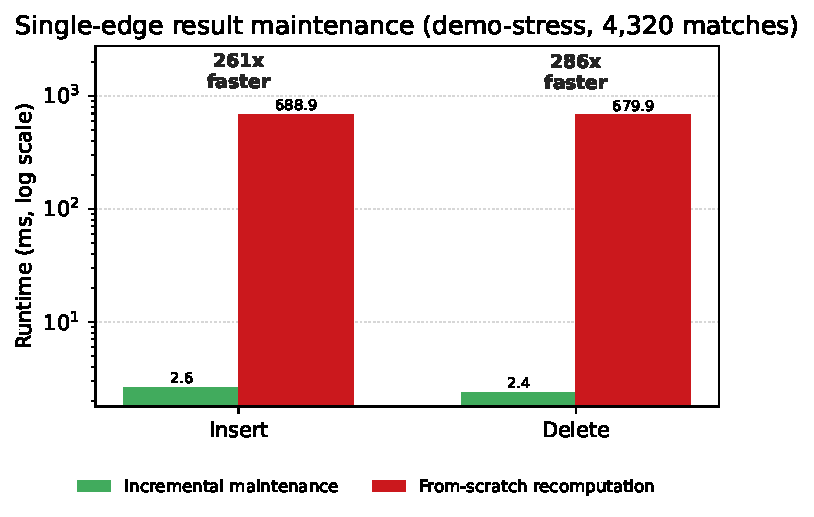
\includegraphics[width=0.6\linewidth]{figures/dynamic_speedup.pdf}
  \caption{Incremental single-edge maintenance vs.\ from-scratch recomputation on the demo-stress graph (log scale). Maintenance cost is governed by the small affected set, not the full result size, giving a two-orders-of-magnitude speedup. Source: \texttt{reports/figures/plot\_dynamic.py} (data \texttt{dynamic\_data.csv}).}
  \label{fig:dynamic}
\end{figure}

The results support three observations. First, correctness holds in every case: the incrementally maintained result set, including the precise added and removed mappings, matches the from-scratch recomputation. Second, the benefit is governed by locality. On the toy graph the incremental method is actually marginally \emph{slower}, because its fixed setup cost (candidate construction and anchor enumeration) dominates when the whole graph has only two matches; this marks the small-input overhead floor. Third, once the result set is non-trivial the advantage becomes decisive (Figure~\ref{fig:dynamic}): on the demo-stress graph the incremental method explores only $6$ partial mappings and finishes in about $2.5$\,ms, whereas recomputing the full result set (all $4{,}320$ mappings) takes roughly $0.68$--$0.69$\,s, a speedup of more than two orders of magnitude. This matches the locality property: the cost of maintenance scales with the size of the affected set $D_e$, not with the size of the full result.

The same harness accepts the real \texttt{.graph} workloads used in the main experiments via \texttt{-{-}input-format graph}, so the table can be extended to Yeast, Human, and HPRD once those datasets are placed under \texttt{data/raw/}. This extension only supports single-edge updates on a fixed query; batched updates, vertex insertion and deletion, and reuse of the recorded partial-mapping structure across successive updates are left as future work. Even in this restricted setting, the experiments show that single-edge result maintenance can be made effectively independent of the total result size.

\section{Optional Extension: Subgraph Homomorphism}
\label{sec:optional-homomorphism}

The final optional extension implements subgraph \emph{homomorphism}, which relaxes the exact-matching semantics of the core reproduction in two ways. Given $G = (V_G, E_G, \ell_G)$ and $Q = (V_Q, E_Q, \ell_Q)$, a subgraph homomorphism is a map $f : V_Q \rightarrow V_G$ such that (a) labels are preserved, $\ell_Q(v) = \ell_G(f(v))$ for all $v$; (b) every query edge maps into the augmented edge set $E_G^+ = E_G \cup \{(w, w) : w \in V_G\}$, that is, $(u, v) \in E_Q \Rightarrow (f(u), f(v)) \in E_G^+$; and (c) $f$ need not be injective, so several query vertices may collapse onto the same data vertex. When endpoints collapse, the induced edge is a self-loop, which $E_G^+$ accepts uniformly, so no conflict arises. Concretely, a query edge $(u, v)$ is satisfied iff $f(u) = f(v)$ or $(f(u), f(v)) \in E_G$.

\subsection{Relationship to Subgraph Isomorphism}

Homomorphism is a strict relaxation of the isomorphism studied in the main report, and the two are connected by a clean identity. Every subgraph isomorphism is a homomorphism, because $E_G \subseteq E_G^+$ and injectivity is a special case. Conversely, because the query graph is loop-free, any two distinct query vertices joined by an edge must receive \emph{different} images under an injective map, so the self-loop case of $E_G^+$ never applies; an \emph{injective} homomorphism therefore satisfies $(f(u), f(v)) \in E_G$ for every query edge and is exactly a subgraph isomorphism. Hence
\[
\mathrm{Iso}(Q, G) \;=\; \{\, f \in \mathrm{Hom}(Q, G) : f \text{ is injective} \,\}, \qquad \mathrm{Iso}(Q, G) \subseteq \mathrm{Hom}(Q, G),
\]
and the additional homomorphisms are precisely the non-injective ones obtained by collapsing query vertices through self-loops. We use this identity as a built-in correctness oracle below.

\subsection{Algorithm}

The homomorphism matcher reuses the backtracking skeleton of the core reproduction with two principled changes. First, the injectivity check is removed: a data vertex may be assigned to more than one query vertex. Second, the edge-feasibility test is evaluated over $E_G^+$: when extending the current partial map with $f(q) = d$, for every already-mapped query neighbor $n$ the pair $(d, f(n))$ is accepted if $d = f(n)$ (a self-loop) or $(d, f(n)) \in E_G$.

A subtle but important consequence is that the label-and-degree (LDF) candidate filter used for isomorphism becomes \emph{unsound} for homomorphism. Because several query neighbors may map to the same data vertex---or to $f(q)$ itself via a self-loop---a low-degree or even isolated data vertex can legitimately host a high-degree query vertex. The matcher therefore uses \emph{label-only} candidates. The reference implementation is \texttt{src/subgraph\_match/homomorphism/} with the experiment harness in \texttt{scripts/run\_homomorphism\_experiment.py}.

\subsection{Correctness Validation}

Correctness is verified at three levels in \texttt{tests/test\_homomorphism\_matcher.py}. First, the matcher output is compared against an independent brute-force oracle that enumerates \emph{all} label-respecting functions $V_Q \rightarrow V_G$ and tests the $E_G^+$ edge constraint directly, on the toy graph and on small cliques. Second, the identity above is checked: the injective subset of the homomorphism results equals the isomorphism results returned by the baseline matcher, and the isomorphisms form a subset of the homomorphisms. Third, edge cases are covered, including collapsing two non-adjacent vertices through a self-loop and mapping an entire triangle query onto a single isolated data vertex (which an unsound degree filter would wrongly reject). All experiments below also report these cross-checks.

\subsection{Experimental Results}

Table~\ref{tab:homomorphism} reports homomorphism counts against isomorphism counts. ``Toy'' uses the $A\!-\!A$ edge query on the debugging graph. ``Hom-demo'' is a deterministic synthetic graph (\texttt{scripts/make\_homomorphism\_demo\_graph.py}) consisting of $15$ disjoint cliques of size $6$, all labeled $A$, queried with the triangle $A\!-\!A\!-\!A$; per clique every one of the $6^3$ vertex assignments is a homomorphism while only $6\cdot 5\cdot 4$ are isomorphisms.

\begin{table*}[t]
  \caption{Subgraph homomorphism vs.\ subgraph isomorphism. ``Injective Hom'' is the injective subset of the homomorphisms and must equal ``Iso''. ``Non-inj.\ Hom'' are the additional non-injective homomorphisms. ``Hom PM'' is the partial mappings explored by the homomorphism search.}
  \label{tab:homomorphism}
  \centering
  \small
  \begin{tabular}{llrrrrrrc}
    \toprule
    Dataset & Query & Hom & Iso & Injective Hom & Non-inj.\ Hom & Hom PM & Hom (ms) & Inj.\ Hom $=$ Iso \\
    \midrule
    Toy & $A\!-\!A$ & 4 & 2 & 2 & 2 & 6 & 0.009 & yes \\
    Hom-demo & $A\!-\!A\!-\!A$ & 3{,}240 & 1{,}800 & 1{,}800 & 1{,}440 & 3{,}870 & 12.32 & yes \\
    \bottomrule
  \end{tabular}
\end{table*}

\begin{figure}[t]
  \centering
  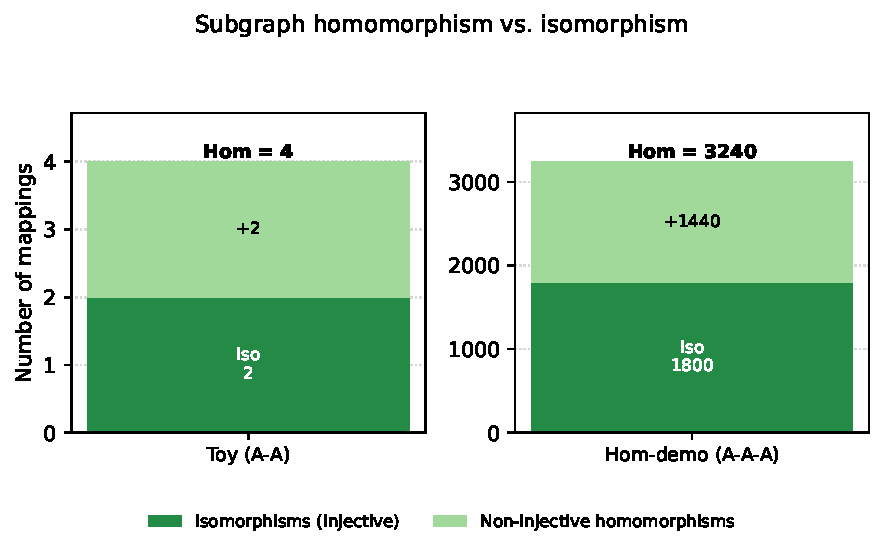
\includegraphics[width=0.72\linewidth]{figures/homomorphism.pdf}
  \caption{Homomorphism counts decompose into the injective part (which equals the isomorphism count) and the additional non-injective homomorphisms produced by the $E_G^+$ self-loop relaxation. Source: \texttt{reports/figures/plot\_homomorphism.py} (data \texttt{homomorphism\_data.csv}).}
  \label{fig:homomorphism}
\end{figure}

The results confirm the theory (Figure~\ref{fig:homomorphism}). In every case the injective subset of the homomorphisms equals the isomorphisms exactly ($2$ on the toy graph, $1{,}800$ on the demo), validating both the homomorphism matcher and, independently, the baseline isomorphism matcher. The relaxation is far from cosmetic: on the toy graph the two non-injective homomorphisms collapse the $A\!-\!A$ query onto a single $A$ vertex through the self-loop, and on the demo the self-loop relaxation produces $1{,}440$ additional homomorphisms on top of the $1{,}800$ isomorphisms ($3{,}240 = 15 \cdot 6^3$ total). Because homomorphism enumerates strictly more mappings and cannot use degree pruning, its search is somewhat heavier than the isomorphism search ($12.32$\,ms vs.\ the baseline's $11.14$\,ms on the demo), which is the expected cost of the broader solution space. This extension is restricted to vertex-labeled, loop-free queries and reuses the same label-only candidate model throughout; combining it with the guard-based pruning of the core reproduction is left as future work.

\section{Conclusion, Development Context, and Reflection}
\label{sec:conclusion}

This project reproduced the core idea of GuP through a correctness-first implementation for exact subgraph matching and organized the report to match the required grading items explicitly. The final report now contains a literature taxonomy, a clear reproduction-scope statement, mandatory experiments on three successful datasets, and a filtering-strategy ablation study.

From the perspective of the development history of subgraph matching, the field has evolved from earlier candidate-space and access-method ideas~\cite{he2008graphql} toward increasingly integrated systems that combine filtering, order optimization, conflict reuse, and execution engineering~\cite{han2019daf,sun2020study,sun2021rapidmatch}. GuP is an instructive modern point in this development line because it emphasizes dynamic, state-aware pruning while remaining conceptually decomposable into interpretable modules.

Our experimental results lead to three final conclusions. First, the project now satisfies the mandatory multi-dataset requirement with successful experiments on \texttt{Yeast}, \texttt{Human}, and \texttt{HPRD}. Second, reservation-based pruning is the only reproduced GuP mechanism that contributes clear and repeated search-space reductions on the current workloads. Third, the current Python prototype still has a visible scalability boundary, which is why \texttt{WordNet} and \texttt{Patents} remain time-boxed boundary datasets rather than full successful result datasets.

The most important lesson for us is that reproducing a research paper is not only about reproducing the same final metric values. It also requires understanding which algorithmic ideas are central, which engineering details control practical performance, and how to report scope boundaries honestly. In this project, the largest gap between the paper and the prototype lies not in correctness, but in the strength of the full guarded candidate-space machinery and the efficiency of the nogood mechanism. This gave us a concrete understanding of the difference between an algorithmic idea that is valid in principle and a system implementation that is competitive in practice.

Overall, we regard the project as a successful course-project-level reproduction of the core GuP method. It demonstrates that guard-based pruning, especially reservation-based pruning, can reduce the search space on real workloads, while also making clear what remains to be improved in a more faithful future reproduction.

\section{Division of Labor}

The project was completed by a two-person team.

\begin{itemize}[nosep]
  \item \textbf{Yi Zha}: framework construction, algorithm reproduction, end-to-end pipeline integration, and report writing.
  \item \textbf{Jinpeng Wang}: algorithm optimization, experimental execution, and presentation slide preparation.
\end{itemize}

Both members jointly participated in the final presentation and oral explanation of the project.


\bibliographystyle{ACM-Reference-Format}
\bibliography{references}

\end{document}
